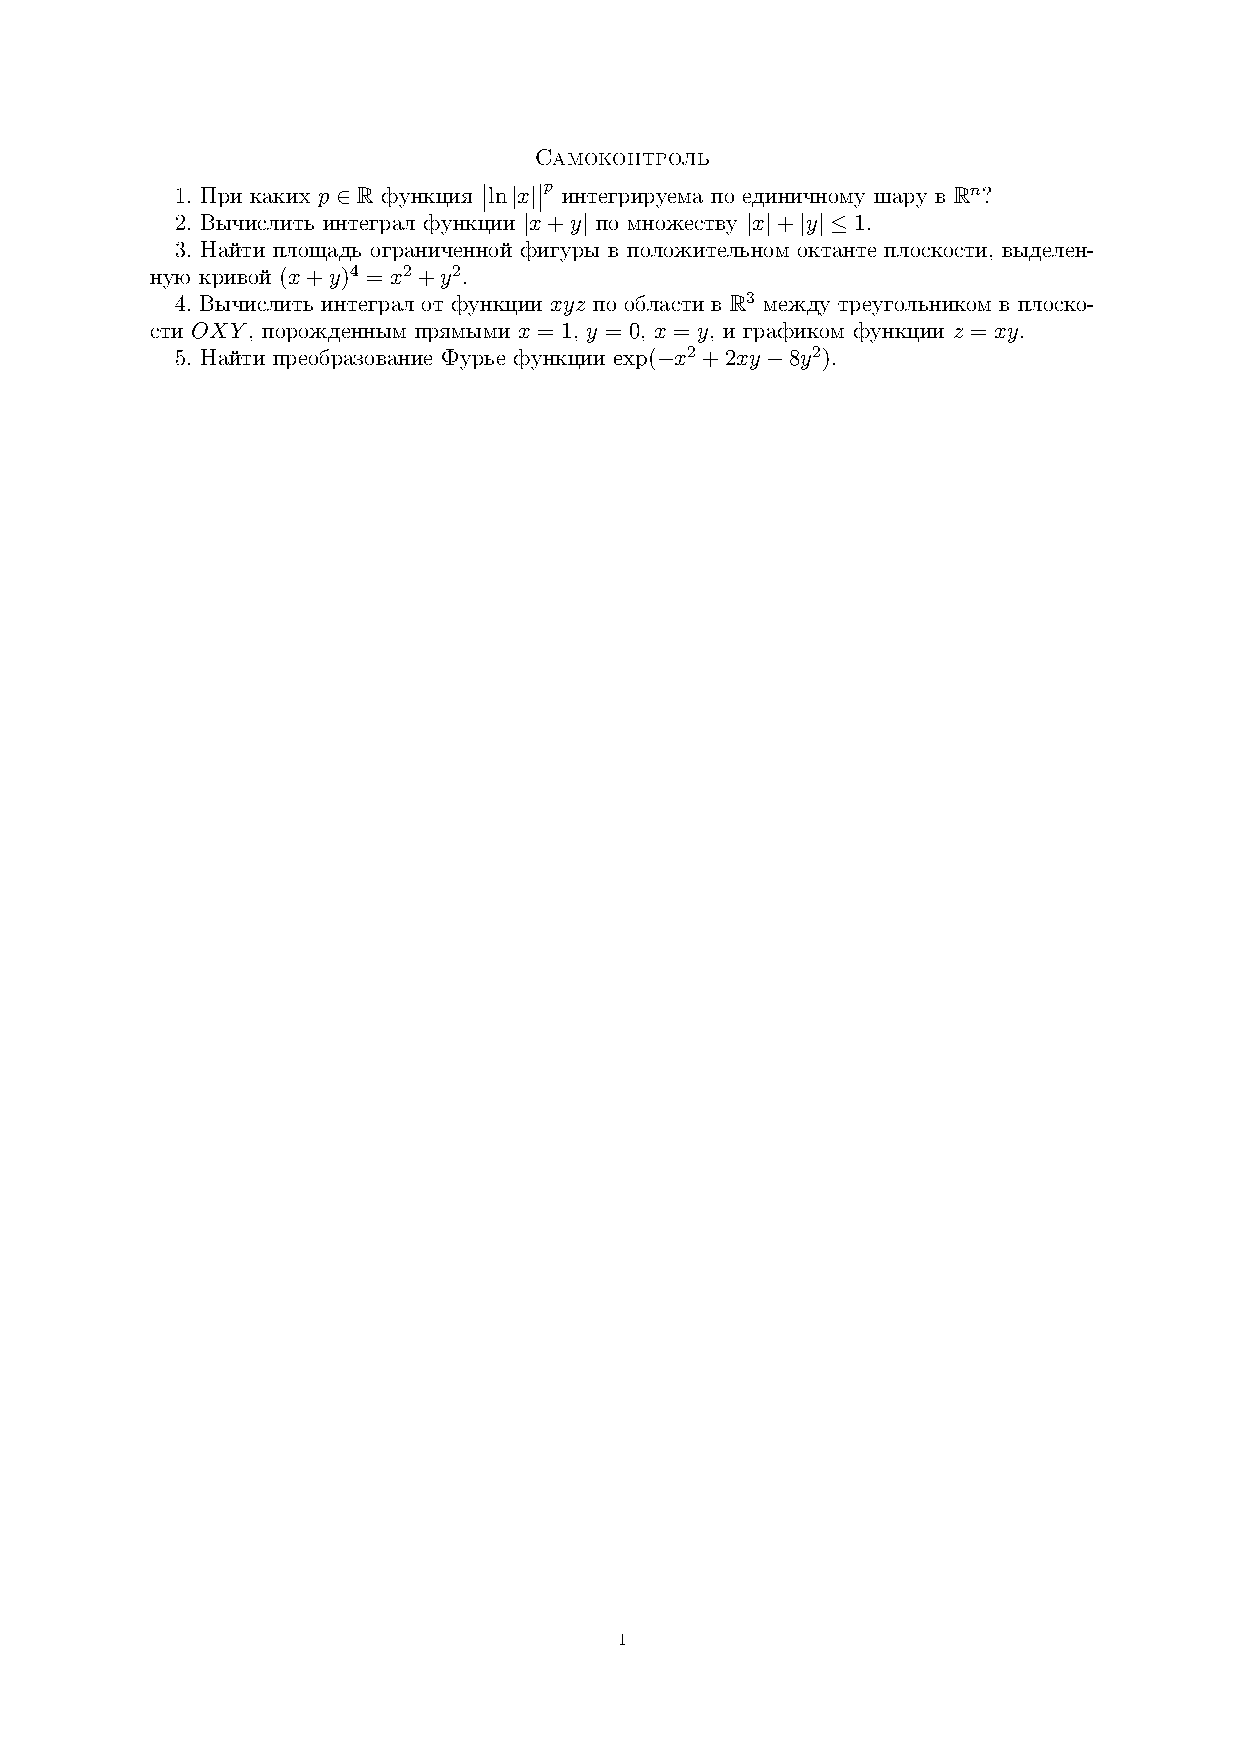
\includepdf{Tasks/self-test1}
\newpage
\section*{Решения}
\subsection*{Задача 1}
	Заметим, что если функция интегрируема по Риману, то она интегрируема и по Лебегу
	\begin{gather*}
	|x|^{p} |\ln|x||^{p} \frac{1}{|x|^{p}}\qquad \text{непрерывно при } |x| < \frac{1}{2}\\
	|x| \cdot \ln|x| \to 0,\ x\to 0
	\end{gather*}
	Введем сферические координаты
	\begin{gather*}
	\begin{cases}
		 x_1 = r \cos(\varphi_1)\\
		 x_2 = r \sin(\varphi_1) \cos(\varphi_2)\\
		 \vdots\\
		 x_n = r \sin(\varphi_1) \ldots \sin(\varphi_{n-1})
	\end{cases}\\
	|J| = r^{n-1} \cdot f(\varphi_1,\ldots, \varphi_{n-1})\\
	\int_{x_1^2 + \ldots + x_n^2 \leqslant 1} |\ln|x||^p dx = \int_{0 \leqslant r \leqslant 1} |\ln(r)|^p \cdot r^{n-1} \int f(\varphi_1, \ldots, \varphi_{n}) d \varphi_1 \ldots d\varphi_{n}\\
	\int_{0}^{1}|\ln(r)|^p r^{n-1} dr = 
	\int_{0}^{\frac{1}{2}} |\ln(r)|^p r^{n-1} dr + \int_{\frac{1}{2}}^{1}|\ln(r)|^p r^{n-1} dr\\
	|\ln(r)| \leqslant c r^{-\alpha}\quad \forall \alpha > 0\\
	\int_{0}^{\frac{1}{2}}|\ln(r)|^p dr \leqslant c^p \int_{0}^{\frac{1}{2}} r^{-\alpha p} dr\\
	\int_{\frac{1}{2}}^{1} \frac{|\ln(r)|^p}{r} dr < \infty\qquad \int_{0}^{\ln(2)} t^p dt < \infty\qquad t = \ln(r)\ \Leftrightarrow\ p > -1\\
	\int_{\frac{1}{2}}^{1} \frac{|\ln(r)|^p}{r} dr = \int_{\frac{1}{2}}^{1} (\ln(r))^{p+1} dr\qquad p > -1
	\end{gather*}
\vskip 0.4in


\subsection*{Задача 2}
	\begin{gather*}
	-1 \leqslant x+y \leqslant 1\qquad -1 \leqslant x-y \leqslant 1\\
	x_1 = x+y,\ y_1 = x-y\\
	\bigg| \frac{\partial(x_1, y_1)}{\partial(x,y)}\bigg| = 
	\begin{vmatrix}
		1 & 1 \\ 1 & -1
	\end{vmatrix}
	=
	-2\\
	\int_{|x| + |y| \leqslant 1} |x + y| dxdy =
	\int_{\substack{|x_1| \leqslant 1 \\ |y_1| \leqslant 1}} |x_1| \frac{1}{2} dx_1 dy_1 =
	\int_{0}^{1} \left(\int_{0}^{1} 2x_1 dx\right) dy =
	2 \int_{0}^{1} dy = 1
	\end{gather*}
\vskip 0.4in


\subsection*{Задача 3}
	\begin{gather*}
	\begin{cases}
		(x+y)^4 = x^2 + y^2\\
		x \geqslant 0\\
		y \geqslant 0
	\end{cases}
	\qquad
	\begin{cases}
		x = r \cos(\varphi)\\
		y = r \sin(\varphi)
	\end{cases}\\
	\begin{cases}
		r^4 (\cos(\varphi) + \sin(\varphi))^4 = r^2\\
		\varphi \in \left[0, \frac{\pi}{2}\right]
	\end{cases}
	\qquad r = \frac{1}{(\cos(\varphi) + \sin(\varphi))^2}\\
	r = \frac{1}{1 + \sin(\varphi)^2} = \frac{1}{2 \left(\sin(\varphi + \frac{\pi}{4})\right)^2}\\
	\int_{0}^{\frac{\pi}{2}} \int_{0}^{\frac{1}{(\cos(\varphi) + \sin(\varphi))^2}} rdr d \varphi =
	\frac{1}{2} \int_{0}^{\frac{\pi}{2}} \frac{1}{(\cos(\varphi) + \sin(\varphi))^4} d \varphi =\\
	\frac{1}{2} \int_{0}^{\frac{\pi}{4}} \frac{1}{\left( \sin(\varphi + \frac{\pi}{4})\right)^4} d \varphi =
	\frac{1}{2} \int_{\frac{\pi}{4}}^{\frac{\pi}{2}} \frac{1}{(\sin(\varphi))^4} d \varphi =\\
	\frac{1}{2} \left(-\frac{1}{3} \operatorname{ctan}(\varphi) \cdot \left(\frac{1}{\sin(\varphi)^2} + 2\right)\right) \bigg|_{\frac{\pi}{4}}^{\frac{\pi}{2}} =
	\frac{1}{6} \cdot 4 = \frac{2}{3}
	\end{gather*}
\vskip 0.4in


\subsection*{Задача 4}
	\begin{gather*}
	x = 1,\ y = 0,\ x = y,\ z = xy\\
	\int xyz dxdydz = 
	\iint_{\substack{y \geqslant 0 \\ y \leqslant x \leqslant 1}} (\int_{0}^{xy} xyz dz) dxdy =
	\int_{y \geqslant 0} \int_{1}^{y} \frac{(xy)^3}{2} dxdy = \int_{y \geqslant 0} \frac{y^7 - y^3}{8}dy
	\end{gather*}
\vskip 0.4in


\subsection*{Задача 5}
	\begin{gather*}
	f = \operatorname{exp}(-x^2 + 2xy - 8y^2) = \operatorname{exp}(-(x-y)^2 - 7y^2)\\
	\hat{f}(y) = (2\pi)^{-\frac{n}{2}} \int_{\mathbb{R}^n} \operatorname{exp} (-i \langle y,x \rangle)f(x) dx\\
	\hat{f}(\lambda, \mu) = \iint_{\mathbb{R}^2} e^{-x^2 + 2xy - 8y^2 - i\lambda x - i\mu y} dxdy =
	\iint_{\mathbb{R}^2} e^{-(x-y)^2 - 7y^2 - i\lambda x - i\mu y} dxdy\\
	u = x-y\qquad v = y\\
	\iint_{\mathbb{R}^2} e^{-u^2 - 7v^2 - i\lambda(u+v) - i\mu v} du dv =
	\int_{\mathbb{R}} e^{-u^2-i \lambda u} du \int_{\mathbb{R}} e^{-7v^2 - i \lambda v - i \mu v} dv
	\end{gather*}
	Тогда
	\begin{gather*}
	\int_{\mathbb{R}} e^{-u^2 - i \lambda u} du = 
	\int_{\mathbb{R}} e^{-(u^2 + i \lambda u - \frac{\lambda^2}{4} + \frac{\lambda^2}{4})} du =\\
	e^{-\frac{\lambda^2}{4}} \int_{\mathbb{R}} e^{-\left(u + \frac{i \lambda}{2}\right)^2} du =
	e^{-\frac{\lambda^2}{4}} \int_{\mathbb{R}} e^{-u^2} du =
	\sqrt{\pi} e^{-\frac{\lambda}{4}}
	\end{gather*}
	Аналогично
	\begin{gather*}
	\int_{\mathbb{R}} e^{-7v^2 - i \lambda v - i \mu v} dv =
	e^{-\frac{(\lambda + \mu)^2}{28}} \int_{\mathbb{R}} e^{-7v^2} =\\
	-(7v^2 + v(i\lambda + i\mu)\sqrt{7} \cdot 2 \cdot \frac{1}{2\sqrt{7}} - \frac{(\lambda + \mu)^2}{28}) - \frac{(\lambda + \mu)^2}{28} =\\
	-\left(\sqrt{7}v + \frac{i(\lambda + \mu)}{2\sqrt{7}}\right)^2 - \frac{(\lambda + \mu)^2}{28} =
	\sqrt{\frac{\pi}{7}} e^{-\frac{(\lambda + \mu)^2}{28}}
	\end{gather*}
	Откуда
	\begin{gather*}
	f(\lambda, \mu) = \frac{\pi}{\sqrt{7}} e^{-\frac{\lambda^2}{4} - \frac{(\lambda+\mu)^2}{28}} =
	\frac{\pi}{\sqrt{7}} e^{-\frac{8\lambda^2 + 2\lambda \mu + \mu^2}{28}}
	\end{gather*}
\vskip 0.4in


